% https://www.overleaf.com/learn/latex/Learn_LaTeX_in_30_minutes
\documentclass[12pt, letterpaper]{article} % doc class - article, report, book
% preamble
\usepackage[utf8]{inputenc} % encoding utf-8

% for graphics
\usepackage{graphicx}
\graphicspath{ {images/} }

% for maketitle
\title{First document}
\author{Flying Cat}
\date{\today}



\begin{document}
	\maketitle % use title, author and date defined above
	
	This is the exercise from 
	\begin{verbatim} 
		https://www.overleaf.com/learn/latex/Learn_LaTeX_in_30_minutes 
	\end{verbatim}

	
	\noindent
	First document. This is a simple example, with no extra parameters or packages included. It's 
	created by \LaTeX{}. This tutorial covers the basic features of documents.
	
	Here is text. Some of the \textbf{greatest} discoveries in \underline{science} were made by 
	\textbf{\textit{accident}}.
	
	Here is graphics.
	
	This is a simple include.
	
	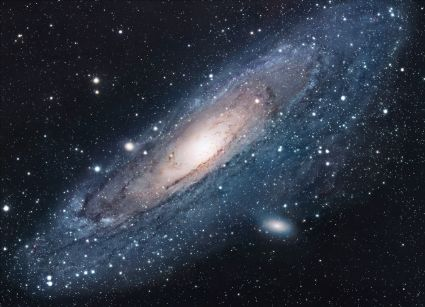
\includegraphics{universe}
	
	This is much better.
	
	\begin{figure}[h] 
		\centering
		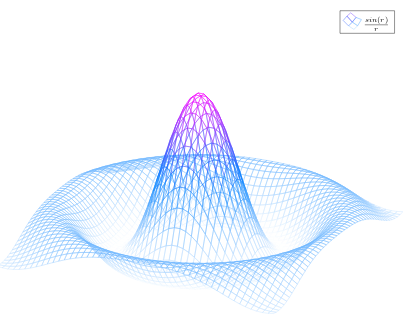
\includegraphics[width=0.5\textwidth]{mesh}
		\caption{a nice plot} % could above or below
		\label{fig:mesh1} % for later referring
	\end{figure}
	
	As you can see in the figure \ref{fig:mesh1}, the function grows near 0. Also, in the page 
	\pageref{fig:mesh1} is the same example.
	
	
\end{document}